% This is lnbip.tex the demonstration file of the LaTeX macro package for
% Lecture Notes in Business Information Processing from Springer-Verlag.
% It serves as a template for authors as well.
% version 1.0 for LaTeX2e
%
\documentclass[lnbip]{svmultln}
\usepackage{graphicx}
\usepackage{makeidx}  % allows for indexgeneration
%\usepackage{graphics} 
% \makeindex          % be prepared for an author index

\def\signed#1{{\leavevmode\unskip\nobreak\hfil\penalty50\hskip2em
  \hbox{}\nobreak\hfil\raise-3pt\hbox{(#1)}%
  \parfillskip=0pt \finalhyphendemerits=0 \endgraf}}

\newsavebox\mybox
\newenvironment{aquote}[1]
  {\savebox\mybox{#1}\begin{quotation}}
  {\signed{\usebox\mybox}\end{quotation}}
%
\begin{document}
%
\mainmatter              % start of the contribution
%
\title{Transitioning Towards Continuous Delivery in the B2B Domain: A Case Study}
%
\titlerunning{Continuous Delivery in the B2B Domain}  % abbreviated title (for running head)
%                                     also used for the TOC unless
%                                     \toctitle is used
%
\author{Olli Rissanen \inst{1,2}, J{\"u}rgen M{\"u}nch \inst{1}
}
\authorrunning{Olli Rissanen}   % abbreviated author list (for running head)
%
%%%% list of authors for the TOC (use if author list has to be modified)
\tocauthor{Olli Rissanen}
%
\institute{Department of Computer Science, University of Helsinki, \\
P.O. Box 68, FI-00014 University of Helsinki, Finland
\and
Steeri Oy, Tammasaarenkatu 5, 00180 Helsinki, Finland
\email{olli.rissanen@aalto.fi, juergen.muench@cs.helsinki.fi}
}

\maketitle              % typeset the title of the contribution
% \index{Ekeland, Ivar} % entries for the author index
% \index{Temam, Roger}  % of the whole volume
% \index{Dean, Jeffrey}

\begin{abstract}        
Delivering value to customers in real-time requires companies to utilize real-time deployment of software to expose features to users faster, and to shorten the feedback loop. This allows for faster reaction and helps to ensure that the development is focused on features providing real value. Continuous delivery is a development practice where the software functionality is deployed continuously to customer environment. Although this practice has been established in some domains such as B2C mobile software, the B2B domain imposes specific challenges. This article presents a case study that is conducted in a medium-sized software company operating in the B2B domain. The objective of this study is to analyze the challenges and benefits of continuous delivery in this domain. The results suggest that technical challenges are only one part of the challenges a company encounters in this transition. The company must also address challenges related to the customer and procedures. The core challenges are caused by having multiple customers with diverse environments and unique properties, whose business depends on the software product. Some customers require to perform manual acceptance testing, while some are reluctant towards new versions. By utilizing continuous delivery, it is possible for the case company to shorten the feedback cycles, increase the reliability of new versions, and reduce the amount of resources required for deploying and testing new releases.

\keywords {Continuous Delivery, Continuous Deployment, Development Process, B2B, Case Study}
\end{abstract}
%
\section{Introduction}
To deliver value fast and to cope with the increasingly active business environment, companies have to find solutions that improve efficiency and speed. Agile practices \cite{cockburn2002agile} have increased the ability of software companies to cope with changing customer requirements and changing market needs \cite{dzamashvili2010impact}. To even further increase the efficiency, shortening the feedback cycle enables faster customer feedback. Continuous delivery is a design practice that aims to shorten the delivery cycles by developing software in a way that it is always ready for releasing.

This study is an exploratory case study, which explores how continuous delivery can be applied in the case company that operates in the B2B domain. While existing studies of applying the practice exist \cite{olsson2012climbing, neely2013continuous}, none of the studies focuses specifically in the B2B domain. This study specifically aims to identify the main requirements, problems and key success factors with regards to continuous delivery in this domain. Extending the development process towards continuous delivery requires a deep analysis of the current development and deployment process, seeking the current problems and strengths. Adopting continuous delivery also requires understanding the requirements of continuous delivery, and restrictions caused by the developed software products. 

This study is organized as follows. The second chapter summarizes the relevant literature and theories to position the research and to educate the reader on the body of knowledge and where the contributions are intended. The third chapter presents the research design. The findings are then presented in the fourth chapter, organized according to the research questions. The fifth chapter interprets the main results, and discusses the limitations of the study. Finally, the sixth chapter summarizes the results of study and answers to the research question, discusses the limitations of the study and introduces further research avenues.

\section{Background and Related Work}
In the agile process software release is done in periodic intervals \cite{cockburn2002agile}. Compared to waterfall model it introduces multiple releases throughout the development. Continuous delivery, on the other hand, attempts to keep the software ready for release at all times during development process \cite{cdbook}. Continuous delivery is an extension to continuous integration, where the software functionality is kept in a state where it can be deployed to production immediately. Production deployments are manually triggered, but the entire deployment process is otherwise automated. While continuous integration defines a process where the work is automatically built, tested and frequently integrated to mainline \cite{duvall2007continuous}, often multiple times a day, continuous delivery adds automated acceptance testing and deployment to a staging environment. The purpose of continuous delivery is that as the deployment process is automated, it reduces human error and documents required for the build, and increases confidence that the build works \cite{cdbook}. It therefore aims to solve the problem of how to deliver an idea to users as quickly as possible.

Continuous delivery differs from continuous deployment. Continuous deployment means that every change goes through the pipeline and automatically gets put into production, resulting in many production deployments every day. Continuous delivery just means that you are able to do frequent deployments but may choose not to do it, usually due to businesses preferring a slower rate of deployment \cite{fowler}. An essential part of continuous delivery is the deployment pipeline, which is an automated implementation of an application’s build, deploy, test and release process \cite{humble2006deployment}. A deployment pipeline can be loosely defined as a consecutively executed set of validations that a software has to pass before it can be released. Common components of the deployment pipeline are a version control system and an automated test suite.

Challenges in adopting continuous delivery have been researched in multiple studies. Olsson et al. investigate the organization evolution path and the transition phase from continuous integration to continuous delivery \cite{olsson2012climbing}. The authors define continuous delivery as one of the final steps in the organization evolution path. The authors identify barriers that companies need to overcome to achieve the transition. One such barrier is the custom configuration at customer sites. Maintaining customized solutions and local configurations alongside the standard configurations creates issues. The second barrier is the internal verification loop, that has to be shortened not only to develop features faster but also to deploy fast. Finally, the lack of transparency and getting an overview of the status of development projects is seen as a barrier.

One of the largest technical challenges is the test automation required for rapid deployment \cite{cdbook, humble2006deployment}. Neely and Stolt found out that with a continuous flow, Sales and Marketing departments lost the track of when features are released \cite{neely2013continuous}. Implementing the deployment infrastructure also requires knowledge from the development and operations team \cite{humble2006deployment}. Another challenge is to sell the vision and reasoning behind continuous delivery to the executive and management level \cite{neely2013continuous}.

\section{Case study}
To provide insight into extending the development process towards continuous delivery, the following research questions have been chosen: \newline

\noindent \textbf{RQ1: What are the B2B specific challenges of continuous delivery?}

\noindent Software development practices and product characteristics vary based on the domain and delivery model. Typical B2C applications are hosted as Software as a Service (SaaS) applications, and accessed by users via a web browser. In the B2B domain, applications installed to customer environments are very common. The purpose of this research question is to identify the challenges faced in applying continuous delivery in the B2B environment. The research question is answered by conducting interviews to discover the current development process and its challenges in the case company, and using these findings and the available literature on continuous delivery to map the initial set of challenges these approaches will encounter in the case company. The available literature is used to provide a thorough understanding of continuous delivery as a whole, so that challenges can be identified in all aspects of the practice.\newline

\noindent \textbf{RQ2: How does continuous delivery benefit the case company?} %What are the problems and strengths of the current development process?

\noindent To rationalize the decision to adopt continuous delivery in a company, the actual benefits to the business have to be identified. This research question aims to identify clear objectives for what is achieved by adopting continuous delivery. Sections of the interview aim to identify the current perceived problems of the case company related to deployment, product development, collecting feedback and guiding the development process. These problems are then compared to the benefits of the approach found from the literature.

\subsubsection{Research design}
In this research, the units under the study are two teams within the case company, and the two software products developed by these teams. By focusing on two different products, a broader view on the application and consequences of the development approach can be gained. The first product, a marketing automation called Dialog, is used through an extensive user interface. The second product under inspection is a Master Data Management \cite{loshin2010master} solution running as an integrated background application. 

%Methods
The primary source of information in this research are semi-structured interviews \cite{runeson2009guidelines}, performed within the two teams under study. The interview consists of pre-defined themes focusing on current development process, current deployment process, current interaction with customers, the software products and future ways with continuous delivery. Data is also collected through the product description documents and development process documents to verifying and supplementing the interview data. 

%Data collection
The interview is a semi-structured interview with a standardized set of open-ended questions, which allows deep exploration of studied objects \cite{runeson2009guidelines}. The interviews are performed once with every interviewee. There are a total of 12 interviewees: 6 in each team. The interviewees in the first team consist of 5 software designers and one team leader. In the second team, the interviewees consist of 3 software designers, a quality assurance engineer, a manager for commercialization and a team leader. Leading questions are avoided on purpose, and different probing techniques such as "What?"-questions are used. The interviews are performed in the native language of the interviewee if possible, otherwise in English, and are recorded in audio format. The audio files are then transcribed into text.

%Data analysis
The data analysis is based on template analysis, which is a way of thematically analysing qualitative data \cite{king1998template}. The initial template was first formed by exploring the qualitative data for two themes: development process and deployment of software. Through multiple iterations of the data, multiple subthemes were then added to the two existing themes by further coding the data. Attention was paid to different roles of the interviewees.

\section{Results}
This section is structured according to the research questions. The challenges regarding continuous delivery are analyzed in three areas: technical, procedural and customer. Technical aspect includes the environmental challenges, configural challenges and other challenges related to the software product and its usage. Procedural aspect includes the challenges regarding the software development process. Customer aspect consists of the customer interaction process and customer commitment.

\subsection{Technical challenges}
The technical challenges for continuous delivery are derived from the interviews. A part of the interview focuses on the current deployment process and customer interaction of the case company. The current deployment process, customer interaction and challenges related to them are then used as a basis for analysing challenges that influence continuous delivery. 

\begin{table}[htb]
    \begin{tabular}{ | p{12cm} |}
    \hline
    \textbf{Specific problem} \\ \hline
    Downtime is critical for certain customers \\ \hline
    Automated testing has to be built on top of a matured software product \\ \hline
    Software is often integrated to multiple third party applications \\ \hline
    Software is often accompanied by multiple external components \\ \hline
    There exists multiple different configurations due to having multiple customers with different specifications \\ \hline
    Transferring the software product to diverse customer-owned environments requires different deployment configurations \\ 
    \hline
    \end{tabular}
    \caption{Technical challenges in continuous delivery.}
    \end{table}

Downtime of the case company's products can be fatal. According to the Dialog product owner, downtime causes end-users being unable to perform their job. Downtime can also interrupt ongoing customer tasks, possibly losing critical data in the progress. Currently the deployment time for both projects is negotiated with the customer to prevent these cases, and the version deployments are done when the system can be closed for a short period of time. 

The developers perceive automated testing and test environments to be the largest technical task. The developers state that building a sufficient test automation is a very laborious process especially due to the maturity of the software, and are concerned with the maintainability of the test suite. The management is not sure what to test with automatic acceptance testing to validate a version. 

Both of the case company's software products are integrated to various third party applications and APIs. Changes to the interfaces communicating with these applications must be planned and discussed in advance. Based on the interview results, automatically updating the integrations requires an unduly amount of work considering the results. 

It is also common for B2B applications to have external components that have to be configured when the software is installed or the APIs to these components changed. The configurations for these external components either have to be manually updated, or automated as well. One of the main differences between B2B and B2C domains is the production environment. Both of the case company's products are used in multiple different customer environments. This introduces a problem of managing different configurations per customer environment and software instance.

\subsection{Procedural challenges}
The procedural challenges are analyzed based on the development process documentations of the company and the interviews. In the interviews, a section is dedicated to the current development process of the case company. The development process and its challenges are then used to analyse and identify challenges that influence continuous delivery.

\begin{table}[htb]
    \begin{tabular}{ | p{12cm} |}
    \hline
    \textbf{Specific problem} \\ \hline
    User acceptance testing environment is a requisite for production release \\ \hline
    The development process drifts towards small feature branches from long-lived feature branches \\ \hline
  Triggering the compilation and deployment of a modular project to maintain integrity is hard \\ \hline
  The software has to be deployed to multiple customers \\ \hline
  Versioning is affected by having different customer profiles of the product \\ \hline
  Responsibility of deploying moves towards developers \\ \hline
  Management and sales loses track of versions \\
    \hline
    \end{tabular}
    \caption{Procedural challenges in continuous delivery.}
    \end{table}


The basic deployment pipeline in the case company first includes a deploy to a user acceptance testing server, which is then tested manually by either the team or the customer. Only after the version has been acceptance tested and validated to work properly, can the production version be released. Continuous deployment to production is seen very risky due to the applications playing a major role in running the customers business. 

Both of the case company's products are developed with a branching model, where feature branches are first thoroughly developed and then integrated to the master branch. With continuous delivery the long-lived feature branches should be changed to short-lived and relatively small feature branches to allow exposing new functionality faster to the customers, and receive feedback faster. While the small feature branches might be common for companies with a relatively new software products, companies that have been developing products for a long time might be more devoted to the practice of long-lived feature branches. %However, it is still possible to 

The software applications in B2B often are large and modular applications, as is the case in the case company. The point when a deployment is triggered has to be designed to maintain the integrity of the application. As the deployment process is currently manually triggered by first releasing a version, a suitable time can be chosen each time. When a production deployment is triggered in continuous delivery, each module has to be in the correct state in order to produce a coherent version.

Both of the case company's products are used by multiple customers, each having their own environments. As the deployments are currently done manually, the customers receiving each deployment can be manually chosen.However, with a continuous delivery process whenever a feature or a new release is ready to be delivered, it can either be deployed to a single customer or to every customer. 

%Versioning
Multiple customer environments affects versioning of the software product. In the case company, each customer has a unique configuration of the product, with possibly different versions of certain components. According to Jan Bosch, in an Innovation Experiment System environment only a single version exists: the currently deployed one. Other versions are retired and play no role \cite{bosch2012building}. However, with multiple environments, multiple different versions of the software are necessary at least in the early phase. 

%Developer responsibility 
Continuous delivery also drifts response towards the developer, and the developers decide what is ready to be released. Currently in the case company the product owners and team leaders are responsible for negotiating the deployment date with the customer, and they also inform the developers that a new version is required. If the developer can single-handedly deploy a feature, the management can quickly lose track on the features available to customers. This also requires the developers to deeply understand the details of the version control system and automated testing. 

Due to increased developer responsibility and varying interval of version updates continuous delivery causes, a team leader expresses concern that the delivery process complicates tracking when deployments are performed, and when features are finished. This also concerns other parties working in the customer interface, such as sales. 

\subsection{Customer challenges}
The customer challenges are analyzed based on two sections of the interview: customer interaction and the deployment process.

\begin{table}[htb]
    \begin{tabular}{ | p{12cm} |}
    \hline
    \textbf{Specific problem} \\ \hline
    Some customers are reluctant towards new versions \\ \hline
    Customers are trained to use a certain version, and modifications confuse the users \\ \hline
    Changelogs are especially important, since as versions are released faster the customers become less aware on what has changed  \\ \hline
    Pilot customer is required for developing the continuous delivery process \\ \hline
    Acceptance testing is performed by both the company and the customers, and requires a lot of resources from the customers \\ \hline
    Production deployment schedule has to be negotiated with the customer \\ \hline
    Ongoing critical tasks by users cannot be interrupted by downtime \\ 
    \hline
    \end{tabular}
    \caption{Customer challenges in continuous delivery.}
    \end{table}

Some customers of the case company are reluctant towards new releases. One of the reasons for this reluctancy is that new releases occasionally contain new bugs. In the case company, customers have been trained to perform certain tasks with a certain user interface. The customer might perform these tasks daily, once every two weeks or even less frequently. If the UI changes often, the customers feel lost and initially take more time to perform the tasks. This causes frustration in the users, and visible changes generally increases the reluctancy customers have towards new versions, unless the changes are significantly improving the user experience.  
\begin{aquote}{Product owner}
"The user interface should be easy to use. Now it's relatively hard to learn. If customers have just learned to perform a task, and we change the UI, the feedback is terrible."
\end{aquote}

Listing the changed features in changelog entries is especially important when releases are made more often. While the changes become smaller the faster versions are released, customers become less aware of when the version will be updated and when features have changed. Currently the version deployments are negotiated with the customers, and when the deployments are made more often, discussions regarding version releases may be reduced or even ceased.

A way to identify the best practices in continuous delivery is to develop the continuous delivery process with a pilot customer. Pilot customer is a company willing to help the company to quickly learn what works and what needs to be improved. The interviewees expressed a desire to first test the continuous delivery process with a single customer that is willing to receive updates in a continuous manner, since the engagement model inevitably differs from the current model.

The acceptance testing is performed in varying ways. Some customers require to perform manual acceptance testing before the product can be deployed into production. Other customers trust the developers to perform the acceptance testing. The technical implementation therefore should make it possible to continuously deploy versions to the user acceptance testing environment, and by the push of a button to the production environment. However, if the versions are deployed to user acceptance testing environment very often, customers might feel encumbered by the amount of required testing. The customers also have to be informed whenever a new version is available to the user acceptance testing environment. Customers might be using the software when a new version is deployed, and the deployment process shouldn't interfere with ongoing usage.

\subsection{Benefits of continuous delivery}
A major problem found in the interviews is that currently the reliability towards new versions is low. The low reliability both increases customers reluctancy towards version updates, and increases the amount of user acceptance testing that is performed after version release. Versions are occasionally forgotten from the UAT phase due to the lack of comprehensive automated testing and the broad scale of features in both software products. These features can then remain broken or contain bugs when the users start using the new version. This is fundamentally caused by the lack of quality assurance before the release. Adopting a test automation solves this issue, as long as tests are written for every feature.

The case company has had problems with the human error factors in manual build processes. Essentially, every each deployment is a new error-prone experiment. This increases the duration required for deploying, and lessens both the reliability and confidence in builds. The human error factor is increased by lacking documentation and parts of the deployment being memorized by developers. With continuous delivery, only a handful of developers might have knowledge of the entire build deployment configuration, but everyone is able to trigger the deployment process. 

The management considers improving the deployment process to be one of the most important improvements. According to the findings, continuous delivery mainly increases the speed, quality, and capacity of the development. Speed and capacity are ensured by automated deployment, while quality is increased by the automated testing and faster feedback. Smaller problems can be quickly fixed without spending unnecessary time on manually deploying a new version to the customer, and bigger changes only take as long as the implementation requires. After the initial investment, the practice will eventually allow the company to spend less money on management and operations, because unnecessary repetitive work and bugs caused by manual building can be eliminated. %D

\section{Discussion}
The results suggest that the challenges faced in continuous delivery in the B2B context are multidimensional, and related to the technical, procedural and customer aspects. The major difference a company operating in the B2B domain faces in the transition as compared to the B2C domain is that there are plenty of customers with unique properties, whose business relies on the software. The primary issues causing these challenges are the diverse customer owned environments and the importance of the software product for the customer. 

%KUVA 1
\begin{figure}[!htb]
  \centering
  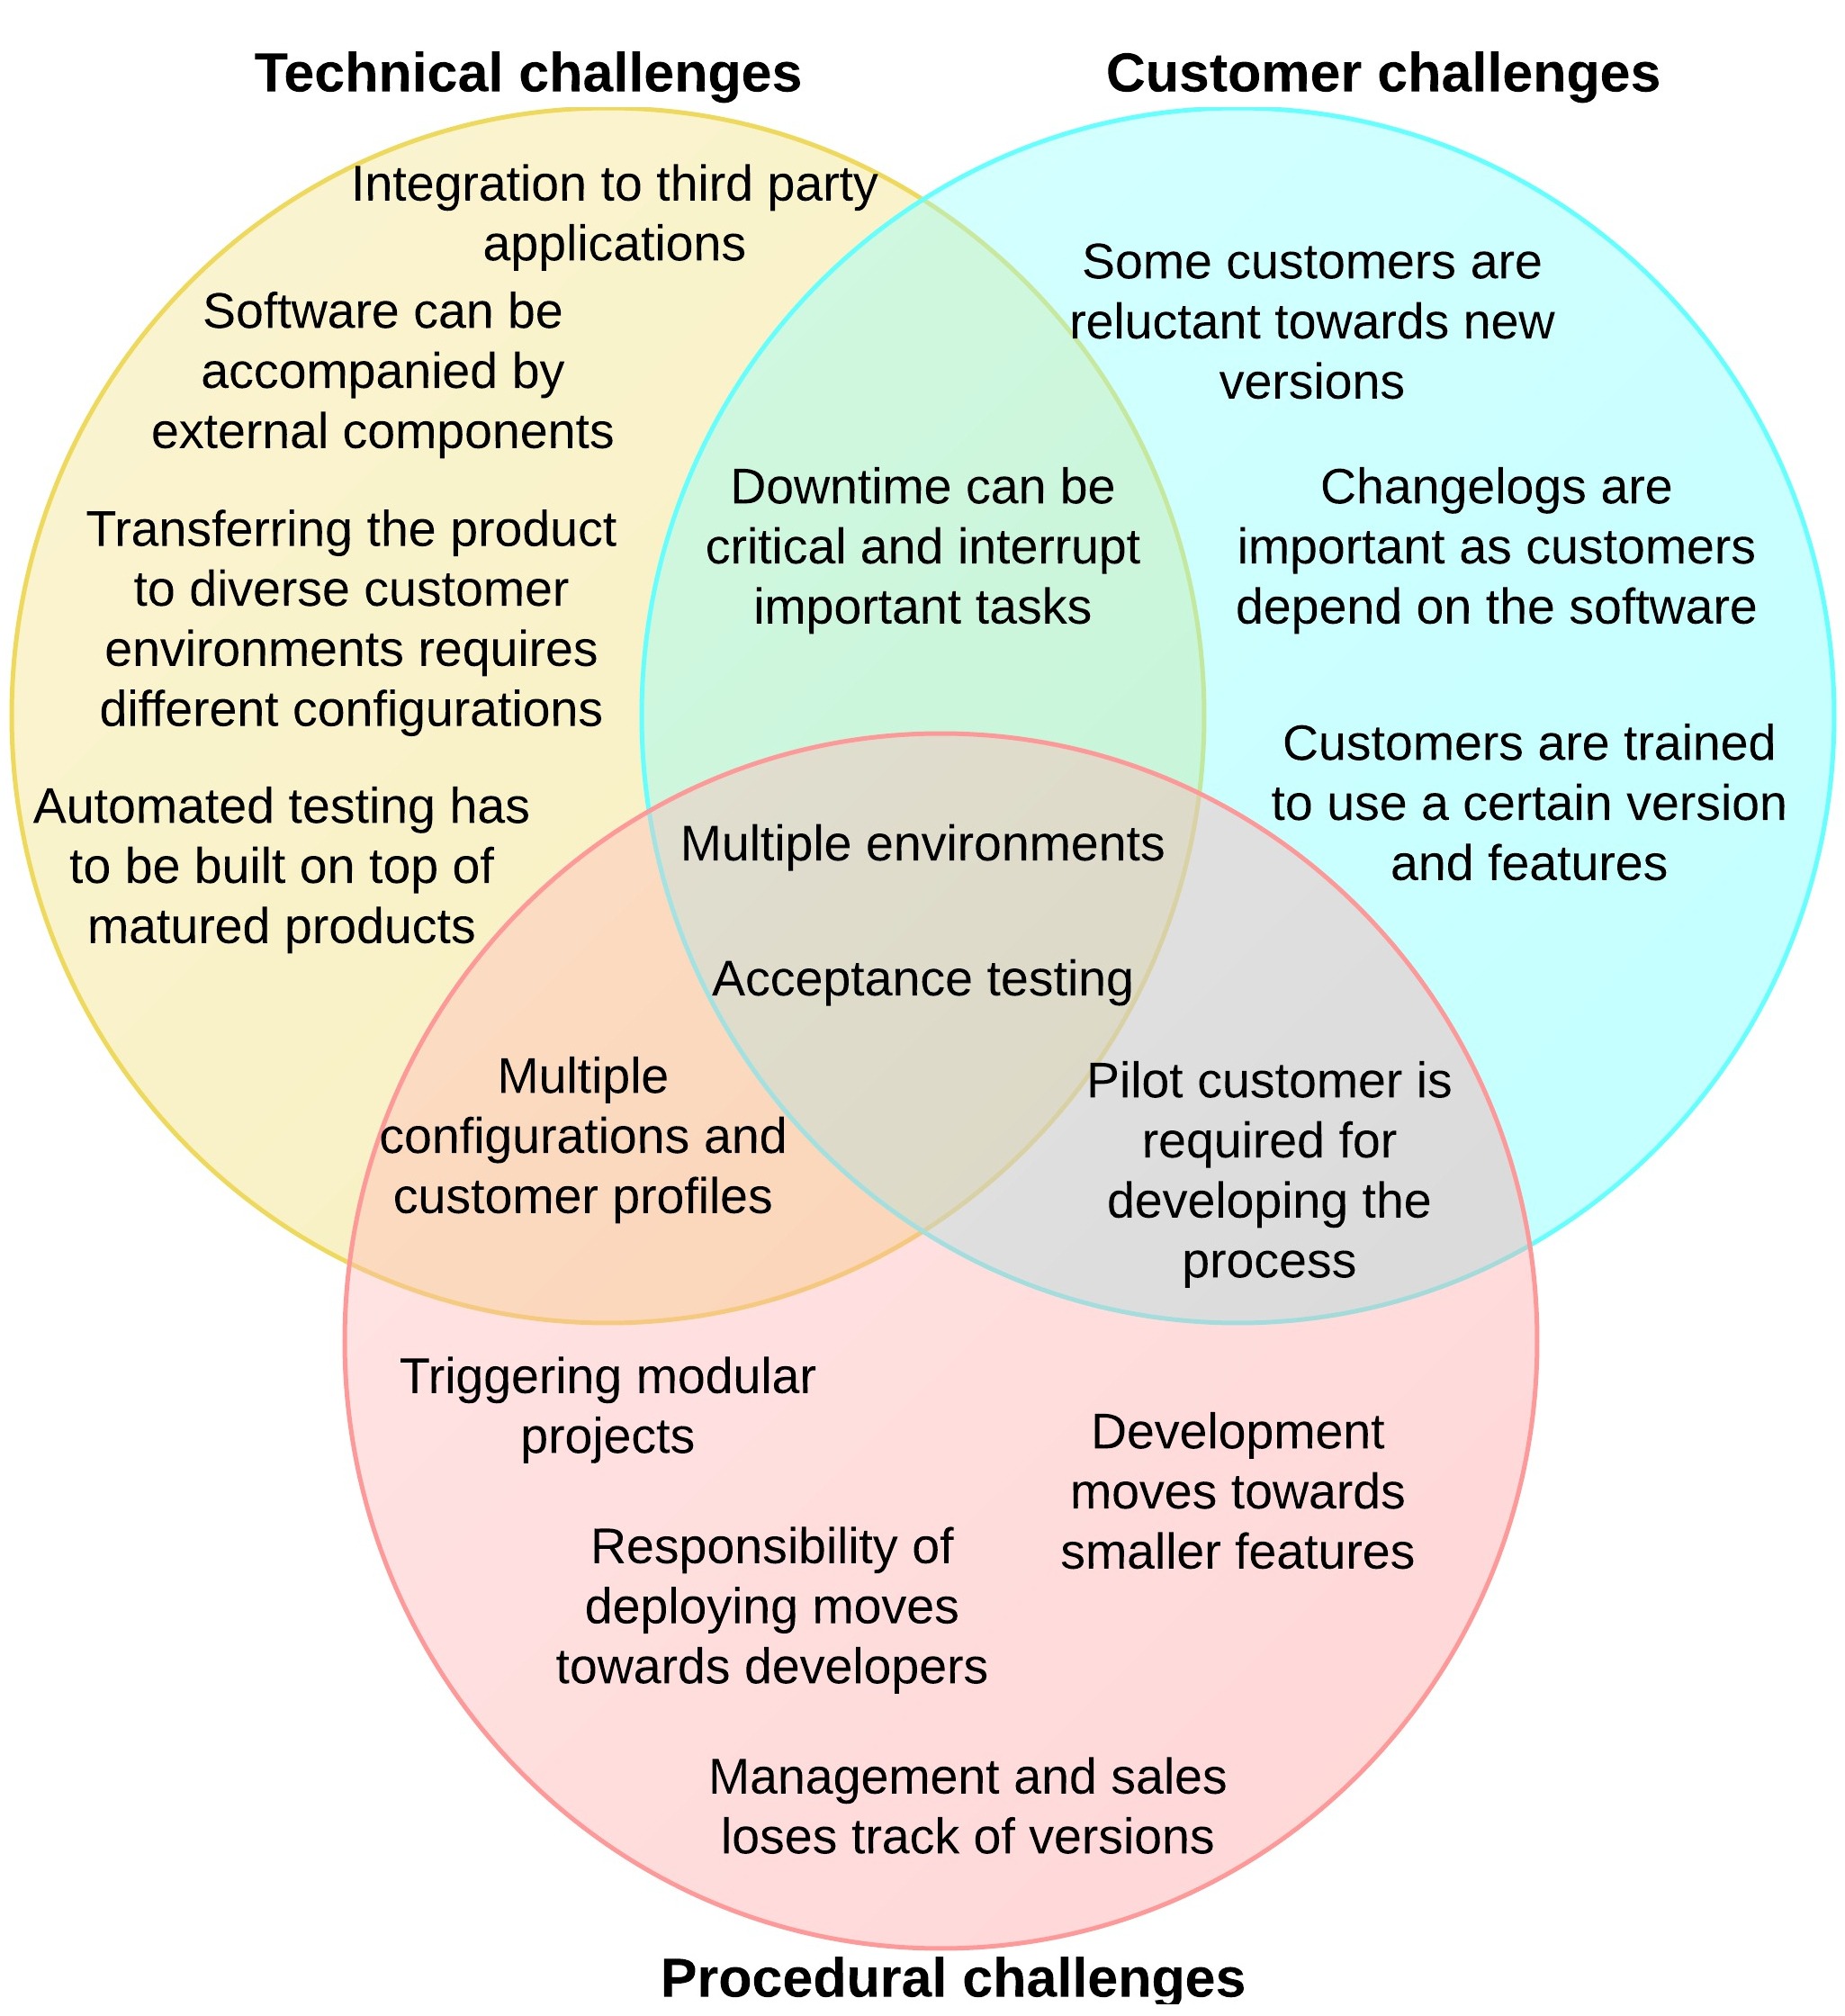
\includegraphics[width=5.0in]{cd_challenges.jpeg}
  \caption{Case company's challenges in continuous delivery.}
  \label{fig1}
\end{figure}

Fig. \ref{fig1} visualizes the challenges the case company faces in transition towards continuous delivery. Multiple challenges are related to two or more aspects, and the problems affecting all aspects can be seen as the core challenges. Acceptance testing is related to all aspects, since customers want to perform acceptance testing with new versions, automated acceptance testing has to be implemented and the user acceptance testing is required before a production release can be made. Another challenge related to all aspects is the diversity of customer environments. It affects the technical implementation, as software has to be transferred to diverse environments. The procedural challenge is that the software has to be deployed to multiple customers, and it has to be decided whether each version is always released to every customer. 

The issues into which the benefits are mapped were found by researching the current deployment process and challenges faced in the development process. An unexpectedly large part of the major issues stated by the interviewees are related to deploying the software, and it was identified as one of the major challenges in the current product development. The benefits found from continuous delivery, which were sought from existing literature \cite{cdbook, neely2013continuous, humble2006deployment}, matched the challenges very well. 

The study also suggests that continuous delivery corresponds to many of the case company's primary needs. The issues related to the deployment process are considered very important by both of the teams. The issues include low reliability of new versions, human error factors when performing version releases and deployments, and long feedback cycles. Additionally, a very large part of the case company's resources are spent on both deploying and testing new versions. One of the main benefits of continuous delivery is that the software is kept in a state where it is always ready for deployment \cite{cdbook}, and that no manual work from the company is required to produce a new version. 

The findings are in align with and could be considered as extending some of the theoretical contributions by Olsson et al. \cite{olsson2012climbing}, who researched the transition towards continuous delivery. Identifying that transitioning towards continuous delivery requires a company to address issues in multiple aspects of the company also benefits companies in practice.   

\subsection{Limitations}
Since case studies only allow analytic generalisations instead of statistical generalisations, the findings cannot be directly generalised to other cases. However, the phenomena was deeply understood through gathering a large amount of qualitative data and systematically analysing it. Therefore the core findings should be applicable to similar research problems outside of the empirical context of this study. This means that the B2B challenges and benefits of continuous delivery can be considered as a starting point for further studies in other contexts where this development model takes place.

Two types of triangulation were used: data triangulation by including persons with different roles into the interviews, and methodological triangulation by collecting documentary data and observations by the author. However, the reliability of the results could have been increased by employing observer triangulation and theory triangulation. 

\section{Summary}
This study was motivated due to lack of studies in continuous delivery focusing on companies operating in the B2B environment. Understanding the central aspects of continuous delivery will be a must for software companies willing to stay ahead of its competitors in the current rapidly moving industry. The findings provide insights into the challenges a company faces in the transition in this domain, and the benefits a company can gain from adopting this practice.

This study has identified the main requirements a company operating in the B2B domain has to address when applying continuous delivery. The challenges can be divided into technical challenges, procedural challenges and challenges related to the customer. These challenges are mostly caused by having multiple customers with diverse environments and unique properties, whose business depends on the software product. While continuously deploying versions to a user acceptance testing environment requires a company to address multiple challenges, continuously deploying to production is even more difficult, since some customers want to perform manual acceptance testing before production releases can be made. 

The benefits of continuous delivery matched to many business problems found in the case company, and a company operating in similar domain with similar products can use them as a basis when considering applying this practice. By utilizing continuous delivery, the case company can solve problems such as long feedback cycles, low reliability in new versions, human error factors and high amount of resources required for deploying and testing new releases. 

\section{Acknowledgements}
We wish to thank the participants of the study for their time and contributions and the reviewers for their valuable comments. We also thank the Finnish technology agency, Tekes, for funding the Cloud Software Factory project, and the Need for Speed program, under which the proposed study was undertaken. This paper is based on thesis work \cite{gradu} completed at the University of Helsinki.

%
% ---- Bibliography ----
%
\begin{thebibliography}{5}

\bibitem{olsson2012climbing} Olsson, H. H., Alahyari, H., \& Bosch, J. (2012, September). Climbing the" Stairway to Heaven"--A Multiple-Case Study Exploring Barriers in the Transition from Agile Development towards Continuous Deployment of Software. In Software Engineering and Advanced Applications (SEAA), 2012 38th EUROMICRO Conference on (pp. 392-399). IEEE.
\bibitem{neely2013continuous} Neely, S., \& Stolt, S. (2013, August). Continuous Delivery? Easy! Just Change Everything (well, maybe it is not that easy). In Agile Conference (AGILE), 2013 (pp. 121-128). IEEE. 
\bibitem{bosch2012building} Bosch, J. (2012). Building products as innovation experiment systems. In Software Business (pp. 27-39). Springer Berlin Heidelberg.
\bibitem{cdbook} Humble, J., \& Farley, D. (2010). Continuous delivery: reliable software releases through build, test, and deployment automation. Pearson Education.
\bibitem{humble2006deployment} Humble, J., Read, C., \& North, D. (2006, July). The deployment production line. In Agile Conference, 2006 (pp. 6-pp). IEEE.
\bibitem{fowler} Fowler, M., ContinuousDelivery, http://martinfowler.com/bliki/Continuous \newline Delivery.html (2015, January)
\bibitem{king1998template} King, N. (1998) Template analysis. In Qualitative methods and analysis in organizational research: A practical guide (pp. 118-134). Sage Publications Ltd.
\bibitem{runeson2009guidelines} Runeson, P., \& Höst, M. (2009). Guidelines for conducting and reporting case study research in software engineering. Empirical software engineering, 14(2), 131-164.
\bibitem{dzamashvili2010impact} Dzamashvili Fogelström, N., Gorschek, T., Svahnberg, M., \& Olsson, P. (2010). The impact of agile principles on market‐driven software product development. Journal of Software Maintenance and Evolution: Research and Practice, 22(1), 53-80.
\bibitem{cockburn2002agile} Cockburn, A. (2000). Agile software development. Cockburn* Highsmith Series Editor.
\bibitem{loshin2010master} Loshin, D. (2010). Master data management. Morgan Kaufmann.
\bibitem{duvall2007continuous} Duvall, P. M., Matyas, S., \& Glover, A. (2007). Continuous integration: improving software quality and reducing risk. Pearson Education.
\bibitem{gradu} Rissanen, O., M{\"u}nch, J. (supervisor), M{\"a}nnist{\"o}, T. (supervisor). Extending the Development Process Towards Continuous Delivery and Continuous Experimentation in the B2B Domain: A Case Study. Master's Thesis. University of Helsinki (2015)

\end{thebibliography}
%
\end{document}
